\chapter{The Second Chapter}
\section*{Methodology}
Random forests are a combination of tree predictors such that each tree depends on the values of a random vector sampled independently and with the same distribution for all trees in the forest(Breiman,2001).The goal of Random forest is creating a predictive model that predicts the value of a target variable bbased on given input variables where one of the input variable is represented by each interior node and the values of the input variable is represented by edges.

\begin{center}
\textbf{Bagging and Random forests}
\end{center}
 
Bagging and random forests use trees as building blocks to constructing more powerful models.

\textbf{Bootstrap}: It is a widely used statistical tool used to quantify uncertainty associated with given estimators. It can easily be applied to a wide range of statistical learning methods even those whose measure of variability is difficult to obtain.

\textbf{Bootstrap aggregation / Bagging}: This is the basic principle behind the training algorithm for random forests which reduces the variance of a statistical learning method.

Consider the set of $n$ independent observations denoted by $C_1,C_2,...,C_3$ each with variance $\sigma^2$. Therefore the variance of the mean $\bar{Z}$ of the observation is given by $\dfrac{\sigma^2}{n}$. Averaging a set of observations reduces the variance.To reduce the variance and increase the prediction accuracy of a statistical learning method, we sample many training sets from the population,build a separate prediction model and average the resulting predictions. Therefore, calculate $\hat{f}^{1}(x),\hat{f}^{2}(x),...,\hat{f}^{B}(x)$ using $B$ separate training sets and average them so as to obtain a single low-variance statistical model given as:

\begin{equation}
\hat{f}_{avg}(x)=\dfrac{1}{B} \sum_{b=1}^{B} \hat{f}^{b}(x)
\end{equation}

However, this is not practical because we cannot have multiple training sets so the bootstrap approach is used where repeated samples from the single training dataset are sampled.In this method, $B$ different bootstrapped training datasets are generated and we train our method on the $b^{th}$ bootstrapped training set to obtain $\hat{f}^{\star b}(x)$ and then average all the predictions to obtain:

\begin{equation}
\hat{f}_{bag}(x)=\dfrac{1}{B} \sum_{b=1}^{B} \hat{f}^{\star b}(x)
\end{equation}

This is called \textbf{bagging}. (When trees are repeatedly fit to bootstrapped subsets of the observations)

So given a training set $X=x_1,...,x_2$ with responses $Y=y_1,...,y_n$, bagging repeats $B$ times and selects random samples \textbf{with replacement} of the training set and fits trees to the sample.Trees are grown deep and are not pruned therefore each individual tree has high variance but low bias.Finding the average of the $B$ trees reduces the variance.

\textbf{How can bagging be extended to a classification problem where $Y$ is qualitative?} Given a test observation, a predicted class can be recorded by each of the $B$ trees and a majority vote is recorded. The overall prediction is the most commonly occurring class among the $B$ predictions.

\begin{center}
\textbf{Out of Bag Error Estimation}
\end{center}

This is a method of estimating the test error of a bagged model without the need of cross validation. Averagely, each bagged tree makes use of around $\dfrac{2}{3}$ of the observation and the other $\dfrac{1}{3}$ of the observation is not used to fit a bagged tree. This observations are referred to as out of bag observation. The response for the $i^th$ observation can be predicted using each of the tree in which that observation was out of bag which will yield around  $\dfrac{B}{3}$ predictions for the $i^th$ observation. To obtain a single prediction for the $i^th$ observation,we take a majority vote of the predicted responses. This gives a single OOB prediction for the $i^th$ observation.

The OOB prediction is obtained for the $n$ observations and the classification error is computed.The OOB error is an estimate for the test error for the bagged model since each of the observation has the response predicted using only the trees that were not fit using that observation. Therefore, the OOB method for test error estimation is convenient when bagging on large datasets. 

%QUOTE HERE
For each observation $Z_{i}=(x_{i},y_{i})$ we build a random forest predictor by averaging the trees corresponding to bootstrap samples in which $z_{i}$ did not appear. The training is terminated when the error stabilizes.

\begin{center}
\textbf{Variable importance measures}
\end{center}

When a large number of trees are bagged, it is no longer possible to represent the statistical learning procedure using a single tree,and it is not also clear which variables are most important to the procedure. Although the collection of bagged trees is difficult to interpret than a single tree, an overall summary of the importance of each predictor can be obtained using the gini index for bagging classification trees.

\textbf{Gini index}: This is the expected error rate of the system.Calculating the gini index for each attribute helps one to get the splitting attributes.


\begin{center}
\textbf{Random Forests}
\end{center}

Random forest is an improvement over bagged trees by providing a small adjustment to the system that decorrelates the trees. In building the decision trees, \textbf{a random sample of m predictors is chosen as split candidates from the set of p predictors} each time a split in a tree is considered. The split is allowed to use only one of those m predictors.

The number of predictors considered at each split is approximately equal to the square root of the total number of predictors, $m\approx \sqrt{p}$. A new sample of $m$ predictors is taken at each split.

Suppose there is one very strong predictor in the dataset and a number of other moderately strong predictors. Then most or all of the predictors will use the strong predictors in the top split in the collection of the bagged trees. Consequently,
all of the bagged trees will look quite similar to each other and therefore the predictions from the bagged trees will be highly uncorrelated. Bagging will not lead to a reduction in the variance over a single tree in this setting.

\textbf{How does random forest overcome this problem?} By ensuring that each split considers only a subset of the predictors.Averagely, $\dfrac{(p-m)}{p}$ of the splits will not consider the strong predictorand the other predictors will have a chance.This is referred to as \textbf{decorrelating the trees}. This approach makes the average of the resulting trees less variable and more reliable.

\textbf{The main difference between bagging and Random Forest} is the choice of the predictor subset size $m$. If a random forest is built using $m=p$, this amounts to bagging. Random Forest using $m=\sqrt{p}$ leads to a reduction in \textbf{test error} and \textbf{OOB} over the bagging technique. It is helpful to use a small value of $m$ when building a random forest if we have a large number of uncorrelated predictors.Random forest does not overfit just like bagging if we increase B.

\begin{center}
\textbf{Implementing the Random forest algorithm}
\end{center}

%\textbf{Data Exploration}.
\begin{enumerate}
\item[•] Loading the Data: The code loads the train(rawdata1) and test(test2) data into the jupyter notebook. The scope of the project is to predict the feature response which are the different categories of risk in the test data.

\begin{verbatim}
raw_data1=pd.read_csv('train.csv')  #loading the train data
test2=pd.read_csv('test.csv')  #loading the test data
\end{verbatim}

\item[•] Shape of the data: The train data is composed of 59,381 observations and 128 features while the test data is composed of 19765 observations and 127 features.

\begin{verbatim}
raw_data1.shape
(59381, 128)
\end{verbatim}

\begin{verbatim}
test2.shape
(19765, 127)
\end{verbatim}

\item[•] To list the features in the data:
\begin{verbatim}
raw_data1.columns.values
\end{verbatim}

\item[•] Factorize string variable: Product Info 2 is a string categorical variable, we transform this feature to enumerate type using the factorize function.The factorize functions returns a list of unique values (or categorical labels) in the product Info 2 column.
\begin{verbatim}
raw_data['Product_Info_2'] = pd.factorize(raw_data['Product_Info_2'])[0]  
raw_data['Product_Info_2']
\end{verbatim}

\item[•] Missing values: From sklearn we import imputer. Where the missing values is Nan, we choose the imputation strategy as mean and the axis is set to 0 meaning that we want to impute the mean values along the columns. The strategy can also be mode incase we replacing categorical missing values. We therefore choose the most occurring value or the median value along the axes.
\begin{verbatim}
imp=Imputer(missing_values='NaN', strategy='mean', axis=0)
imp.fit_transform(raw_data,y='Response')
\end{verbatim}

\item[•] Splitting the data into into train and test.

From sklearn we import model selection which splits the dataset into random train and test subsets.

Test size: Gives the proportion of the dataset that is included in the test split.

Random state: Pseudo-random number generator state that is used for random sampling. 

\begin{verbatim}
train_raw, test_raw=model_selection.train_test_split(raw_data,
test_size=0.4, random_state=100)
\end{verbatim}

\item[•] To prepare the data for modelling, we drop the features 'Id' and 'Response'.

\begin{verbatim}
t1=train_raw.drop(0,axis=1)    #Train_raw dataset
t2= test_raw.drop(0,axis=1)     #Test_raw dataset
t1=t1.drop(127,axis=1)
t2=t2.drop(127,axis=1)
\end{verbatim}

\item[•] Assigning the response and explanatory variables to numpy array.


\begin{verbatim}
ob=list(t1.columns)
def choose_columns(data):
    ret_X= np.array(data.loc[:,ob]) #Explanatory variables
    ret_Y=data.values[:,-1]
    return ret_X, ret_
\end{verbatim}

\item[•] We model the data using the Random Forest algorithm.

From sklearn.ensemble we import the RandomForestClassifier.

\begin{verbatim}
import sklearn.ensemble as en
RF= en.RandomForestClassifier(n_estimators= 250, criterion='gini',
   max_depth=None,min_samples_split=2, min_samples_leaf=1,max_features='auto',   
   max_leaf_nodes=None, min_impurity_split=1e-08,bootstrap=True,            
   oob_score=False,n_jobs=1, random_state=None, verbose=0,warm_start=True)
\end{verbatim}
Description of the parameters that i tuned for the best score.

n\_estimators: The number of trees in the forest.

Criterion: "gini", measures the quality of a split.

max\_depth: The maximum depth of the tree.Takes on integer values or none.If the value is none, then all nodes are expanded until all leaves are pure.

Min\_samples\_split: Minimum number of samples required to split an internal node.

Min\_samples\_leaf: The minimum number of samples required to split an internal node.

Max\_features: Number of features to consider when looking for the best split. If it is auto, then the max features is equal to the sqrt(n features).

Max\_leaf\_nodes: This parameter grows trees with max leaf nodes in the best first fashion.

Min\_impurity\_split: This is the threshold for early stopping in the tree growth. A node will split if its impurity is above the threshold, otherwise it is a leaf.

Bootstrap: It takes on boolean with default =True. If true, the algorithm makes use of bootstrap samples when building the trees.

Oob\_score: It takes on boolean with default =True. If true, the algorithm uses the out of bag samples to estimate the generalization accuracy.

n\_jobs: Default=1. The number of jobs that should run in parallel for bothfit and predict. If -1, then the number of jobs is set to the number of cores.

Random state: If none, it means that the random number generator is the random state instance  used by np.random.

Verbose: Default=0. Controls the verbosity of the tree building process. That is if the verbose is set to a higher number, more information about the tree building process will be seen.

Warm\_start: bool,(default=False). When set to true,the solution of the previous call to fit and add more estimators to the ensemble is reused. Otherwise, just fit a whole new forest.

\item[•] Fit the Random Forest classifier on the train data.

\item[•] Then predict the response feature for the test data that was split using the model selection code. 

\item[•] The same feature transformations are done on the test data provided by kaggle. This is the data we are supposed to predict the response variable and evaluate the score using the quadratic weighted kappa metric.
\end{enumerate}
 \textbf{Quadratic weighted kappa metric}: It can be used to quantify the amount of agreement between the predictions from an algorithm and some trusted labels of the same objects in machine learning. It is a chance adjusted index of agreement and measures the agreement between two ratings.

Calculation of quadratic weighted kappa metric.
\begin{enumerate}
\item[•] We construct an $N\times N$ histogram matrix $O$.$O_{ij}$ corresponds to the number of applications which received a rating $i$ by A and $j$ by B.

\item[•] We calculate an $N\times N$ matrix of weights ,$w$, based on the difference between the rater's score.

\begin{equation}
w_{ij}=\dfrac{(i-j)^2}{(N-1)^2}
\end{equation}

\item[•] An $N\times N$ histogram matrix of expected ratings, E, is calculated, making the assumptions that there is no correlation between the rating scores. This is calculated as the outer product between each rater's histogram vector of ratings and normalized such that E and O have the same sum.

\item[•] The quadratic weighted kappa is calculated from these three matrices as:

\begin{equation}
\dfrac{1-\sum_{ij}w_{ij}o_{ij}}{\sum_{ij}w_{ij}E_{ij}}
\end{equation}

The metric works well for a highly imbalanced classification task. The metric varies from 0 (random agreement) to 1 (complete agreement).In case there is less agreement between the raters than expected by chance, this metric may go below 0. The data has 8 possible ratings and each application is characterized by a tuple (ea,eb), that corresponds to the scores by rater A, actual risk and rater B, predicted risk. 
\end{enumerate}

My predictions on kaggle scored \textbf{0.53074}.

\textbf{Weakness of Random forest}
\begin{enumerate}
\item[•] Random forest may overfit noisy datasets

\item[•] Having a large number of trees makes the algorithm slow for real time prediction
 
\end{enumerate}

To improve my score on kaggle, I employed the Xgboost algorithm whose full name is eXtreme Gradient Booosting. It is a variant of gradient boosting, which is a tree model based supervised learning algorithm. Unlike fitting a single large decision tree to the data, which could amount to overfitting, the boosting approach instead learns slowly. It includes an efficientlinear model solver and a tree learning algorithm.


\begin{center}
\textbf{Xgboost Algorithm}
\end{center}

The full name is eXtreme Gradient Boosting. It is a variant of gradient boosting, a tree model based supervised learning algorithm. It includes an efficient model solver and a tree learning algorithm. This boosting approach learns slowly unlike fitting a large decision tree to the data which likely amounts to overfitting the data.

\textbf{Features of Xgboost}
\begin{enumerate}
\item[•] Customization: Xgboost supports customized objective function and evaluation function.

\item[•] Sparcity: Xgboost accepts sparse input for both the tree andlinear booster, and is optimized for sparse input.

\item[•] Input type: Xgboost takes several types of input data. The recommended type is xgb.Dmatrix.

\item[•] Speed: It can automatically do parallel computation and faster than gradient boosting machine.

\item[•] Performance: Has better performance on different datasets.
\end{enumerate}

\textbf{XG Boost paramers}

The parameters can be grouped into:
\begin{enumerate}
\item[1] General parameters.

Under general parameters we have number of threads.

\item[2] Booster parameters.
\begin{itemize}
\item Stepsize
\item  Regularization
\end{itemize}
       
\item[3] Task parameters.

\begin{itemize}
\item[•] Objective
\item[•] Evaluation metric
\end{itemize}
\end{enumerate}

\begin{center}
\textbf{Model Specification}
\end{center}

%Take this section next to the code and continue with description of rest.
General parameters.
\begin{itemize}
\item nthread: Number of parallel threads.

\item Booster: 
  \begin{itemize}
  \item[•] gblinear: linear function.
  \item[•] gbtree: tree based model.
  \end{itemize}
\end{itemize}
%\textbf{Parameters for tree booster}

\textbf{Implementing the XGBoost algorithms}
\begin{enumerate}

\item[•] \begin{verbatim}
def eval_wrapper(yhat, y):  
    y = np.array(y)
    y = y.astype(int)
    yhat = np.array(yhat)
    yhat = np.clip(np.round(yhat), np.min(y), np.max(y)).astype(int)   
    return quadratic_weighted_kappa(yhat, y)
\end{verbatim}

This function calculates the quadratic weighted kappa metric.

np.clip: Takes three arguments (np.clip(a, a min, a max, out=None)). It clips (limits) the values in an array. Given an interval, values outside the interval are clipped to the interval edges.

np.round: (a,decimals=0,out=None). Evenly rounds to the given number of decimal places.

\item[•] \begin{verbatim}
def get_params():
    
    params = {}
    params["objective"] = "reg:linear"     
    params["eta"] = 0.05
    params["min_child_weight"] = 360
    params["subsample"] = 0.85
    params["colsample_bytree"] = 0.3
    params["silent"] = 1
    params["max_depth"] = 7
    plst = list(params.items())

    return plst
\end{verbatim}

This code sets up a dictionary of parameters for the tree booster.
Objective
\begin{itemize}
\item "reg:linear": default option, Linear regression.

\item "binary: Logistic": Outputs probability. It performs logistic regression for binary classification.

\item "multi:softmax": Uses the softmax objective for multiclass classification.
\end{itemize}

Eta/Learning rate: We can directly get weights of new features after each boosting step. Eta shrinks the feature weights and makes the boosting process more conservative.
Eta is the stepsize shrinkage used in update to prevent overfitting. It is in the range of [0,1], the default is 0.3.

Min\_child\_weight: This is the minimum sum of instance weight needed in a child. It ranges from [0,$\infty$] and the default is 1.

The tree building process will give up further partitioning if the tree partition step results in a leaf node with the sum of instance weight less than the Min\_child\_weight.

Subsample: It is the subsample ratio of the training instance. Setting it to 0.5 means that XGBoost randomly samples half of the data instances and grows trees thus prevents overfitting. It ranges from (0,1], the default value being 1. This parameter makes the model more robust and avoids overfitting.

colsample\_bytree: This is the subsample ratio of columns when constructing each tree. The range is (0,1] and the default is 1. Both subsample and colsample\_bytree cannot be set to 0.

Silent: The default=0. 0 means printing running messages, 1 means silent mode.

max\_depth: This is the maximum depth of a tree. Increasing the max\_depth value makes the model more complex and more likely to overfit. The range is from [1,$\infty$], the default is 6. 

\item[•] \begin{verbatim}
def score_offset(data, bin_offset, sv, scorer=eval_wrapper):
    # data has the format of pred=0, offset_pred=1, labels=2 in the first dim
    data[1, data[0].astype(int)==sv] = data[0, data[0].astype(int)==sv] +   
     bin_offset
    score = scorer(data[1], data[2])
    return score
\end{verbatim}
\end{enumerate}




\newpage
A plot of the feature importances lists the most important features in descending order.
 
\vspace{1pc}
\begin{figure}[hh!]
\caption{Feature Importance}
%\centering
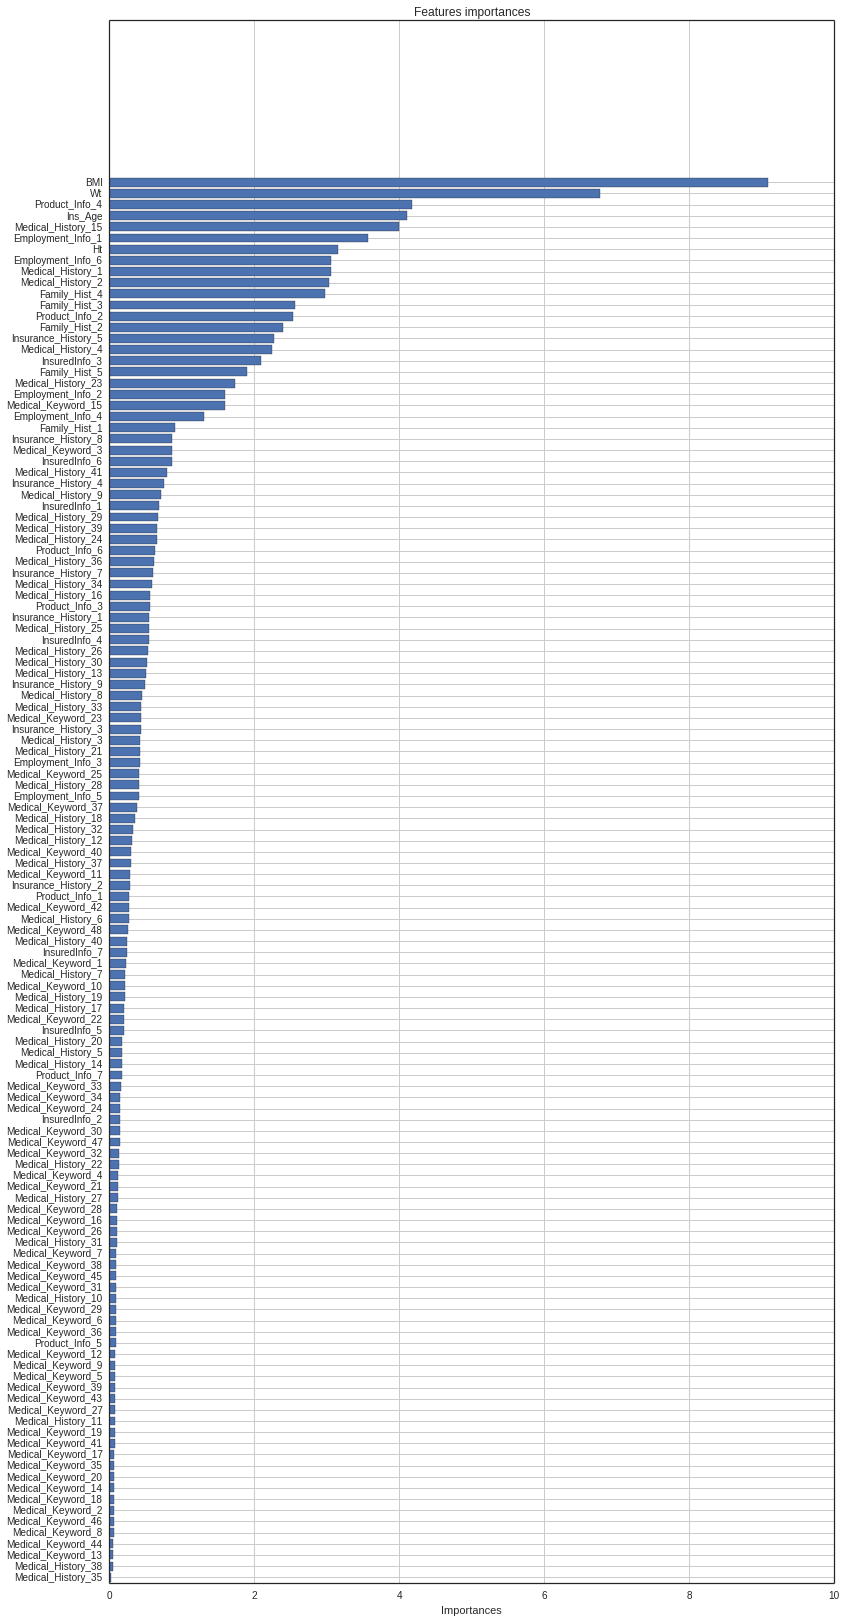
\includegraphics[scale=0.2]{index.png}
\end{figure}

The figure above is a variable importance plot for the insurance data.Variable importance is computed using the mean decrease in the gini index and expressed relative to the maximum.

The code below outputs the five most important and least important variables in ascending order respectively.

\begin{verbatim}
importances =pd.DataFrame({'features' :m.columns,
                           'importances' : RF.feature_importances_})
importances.sort_values(by='importances',ascending=False).head(5)
importances.sort_values(by='importances',ascending=False).tail(5)
\end{verbatim}

\begin{tabular}{|c|c|}
\hline 
\multicolumn{2}{|c|}{The first 5 important predictors} \\ 
\hline 
BMI & 0.089700 \\ 
\hline 
Wt & 0.068185 \\ 
\hline 
Product info 4 & 0.041591 \\ 
\hline 
Ins Age & 0.040372 \\ 
\hline 
Medical History & 0.039763 \\ 
\hline 
\multicolumn{2}{|c|}{The last 5 less important predictors} \\ 
\hline 
Medical History 35 & 0.000219\\
\hline 
Medical History 38 & 0.000512 \\ 
\hline 
Medical History 13 & 0.000551 \\ 
\hline 
Medical History 44 & 0.000612 \\ 
\hline 
Medical History 8 & 0.000622 \\ 
\hline 
\end{tabular} 

\begin{center}
\textbf{Data Visualization}
\end{center}

The scatter plot below shows the relationship between the various responses and the normalized Ins Age.

\begin{figure}[hbtp]
\caption{Scatter plot af Age Vs Response}
\centering
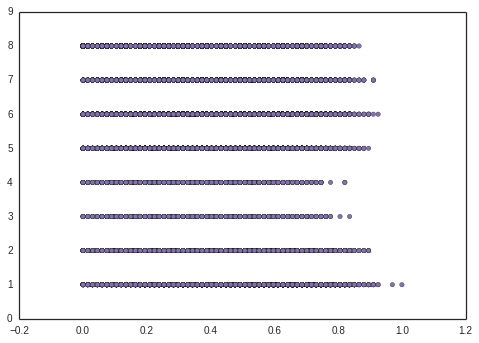
\includegraphics[scale=0.5]{Scatterplot.png}
\end{figure}

The response classes are imbalanced as shown in the plot below.

\begin{figure}[hbtp]
\caption{Class Imbalance of the response variable}
\centering
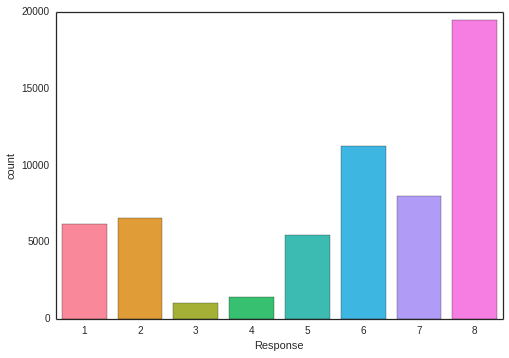
\includegraphics[scale=0.5]{classimbalance.png}
\end{figure}

Visualization of various feature plots.
\begin{figure}[hh!]
  \centering
  \begin{subfigure}[b]{0.4\textwidth}
     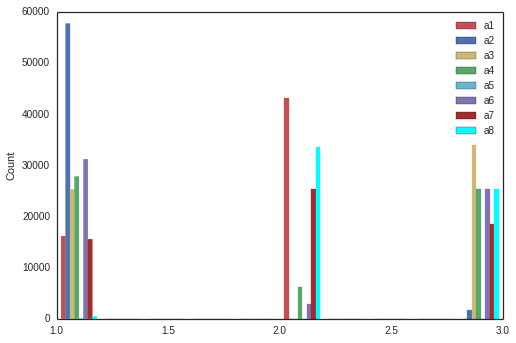
\includegraphics[width=\textwidth]{Insurancehist.png}
     \caption{Insurance history plot}
     \label{imbalance}
  \end{subfigure}
  \quad
   \begin{subfigure}[b]{0.4\textwidth}
      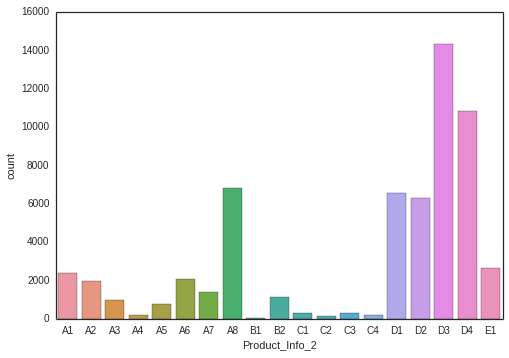
\includegraphics[width=\textwidth]{categoricalplot.png}
      \caption{Product Info 2}   
   \end{subfigure}
   \caption{Feature data plots}
\end{figure}

\begin{figure}[hh!]
  \centering
  \begin{subfigure}[b]{0.4\textwidth}
     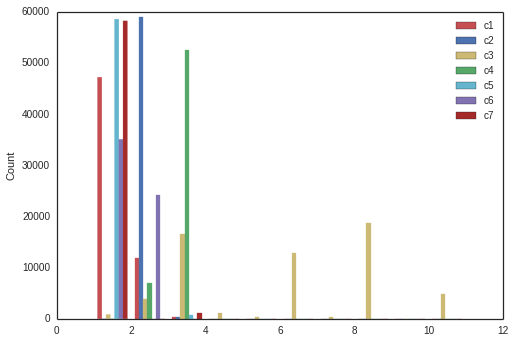
\includegraphics[width=\textwidth]{Insuranceinfo.png}
     \caption{Insurance information plot}
     \label{imbalance}
  \end{subfigure}
  \quad
   \begin{subfigure}[b]{0.4\textwidth}
      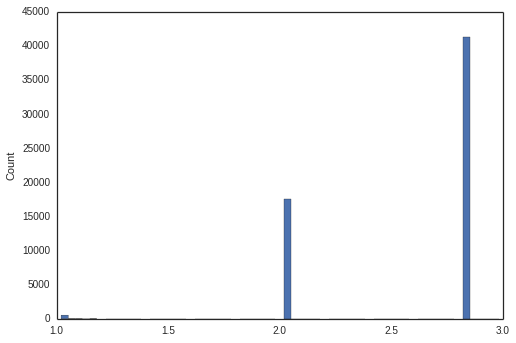
\includegraphics[width=\textwidth]{Familyhist.png}
      \caption{Family history plot}   
   \end{subfigure}
   \caption{Feature data plots}
\end{figure}

\begin{figure}[hh!]
  \centering
  \begin{subfigure}[b]{0.4\textwidth}
     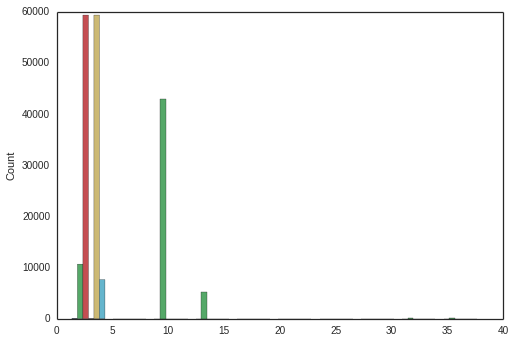
\includegraphics[width=\textwidth]{EmploymentInfo.png}
     \caption{Employment information plot}
     \label{imbalance}
  \end{subfigure}
  \quad
   \begin{subfigure}[b]{0.4\textwidth}
      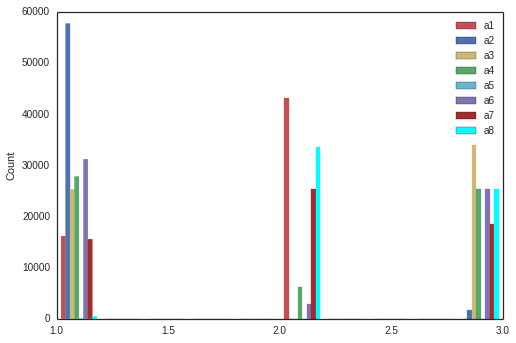
\includegraphics[width=\textwidth]{Insurancehist.png}
      \caption{Insurance history plot}   
   \end{subfigure}
   \caption{Feature data plots}
\end{figure}



%Text text text text text text text text text text text text text text
%text text text text text text text text text text text text text text.
%
%When you get stuck, don't panic. 
%The world is unlikely to end just now. 
%Remember you can consult your supervisor, tutor, and Blaise at agreed times. 
%
%\begin{thm}[Jeff's Washing Theorem]
%\label{thm:jwt}
%If an item of clothing is too big, then washing it makes it bigger;
%but if it is too small, washing it makes it smaller.
%\end{thm}
%\begin{proof}
%Stated without proof. But a proof would look like this. 
%\end{proof}
%
%Notice that no Lemmas are required in the proof of Theorem \ref{thm:jwt}.
